\documentclass[12pt, a4paper]{article}
\usepackage[utf8]{inputenc}
\usepackage[T1]{fontenc}
\usepackage{fullpage}
\usepackage{hyperref}
\usepackage[parfill]{parskip}
\usepackage{natbib}
\usepackage{url}
\usepackage{amsmath}
\usepackage{graphicx}
\graphicspath{{images/}}
\usepackage{vmargin}
\usepackage[nottoc,numbib]{tocbibind}


\title{Lab Assignment 2: Where’s Croc}	% Title
\author{André Le Blanc, Joel Wallin}
\date{\today}			

\makeatletter
\let\thetitle\@title
\let\theauthor\@author
\let\thedate\@date
\makeatother

%----------------------------------
% Wizard stuff
%----------------------------------
\begin{document}

\begin{titlepage}
	\centering
    \vspace*{0.5 cm}
    %\includegraphics[width=5cm,height=5cm,keepaspectratio]{deadrop_text.png}\\[0.5 cm]
    %\includegraphics[width=5cm,height=5cm,keepaspectratio]{deadrop_logo.png}\\[1 cm]
    %\textsc{\huge Artificial Intelligence (1DL340) fall 2016}\\[2.0 cm]
	%\textsc{\Large \today}\\[0.5 cm]
	\rule{\linewidth}{0.2 mm} \\[0.4 cm]
	{ \huge \bfseries \thetitle}\\  
	\rule{\linewidth}{0.2 mm} \\[1.5 cm]
    \includegraphics[width=10cm,height=10cm,keepaspectratio]{crocD.jpg}\\[0.5 cm]
    
    \textsc{\Large Lab Group 14:}\\[0.5 cm]
	\begin{minipage}{0.4\textwidth}  
    \begin{align*}
	&\text{André Le Blanc}    &&\text{910930-3850}\\
	&\text{Joel Wallin}  &&\text{941123-3134}\\
	\end{align*}
	\end{minipage}\\[2 cm]
\end{titlepage}


\newpage
\tableofcontents
\newpage

\section{Introduction}

In this lab assignment the task was to guide a park ranger to a crocodile. The crocodile can hide in any of forty water holes in the area. We do not know if he is in a specific waterhole unless the park ranger searches that water hole. The crocodile moves between the water holes meaning that the crocodile could be in a waterhole that we have searched previously. 

Luckily there is information about the average value and standard deviation of salinity, nitrogen and phosphate in every water hole. The crocodile is also equipped with a sensor which at every step in the program has the current measured value of salinity, nitrogen and phosphate. With this information a hidden Markov model was used to find the crocodile.

\subsection{Tools used for the project}

The program is written in R, a high level multiparadigm language designed for statistical computing. RStudio is used as the development environment and Git/Github for version control. 

\section{Algorithms}

Evaluating the probability that the crocodile is at a given node is done with the help of a hidden Markov model (HMM). And the forward algorithm is used to predict at which node it is most likely that the crocodile is. But in order to do that accurately, the HMM has to take the nature of the problem space into account.

\subsection{Hidden Markov models}

A hidden markov model is a model where the system that is being modeled is a Markov chain. A Markov chain is a memoryless stochastic process. This means that you can make predictions about future states solely based on the current states that are as accurate as if you knew what the previous states were. %I don't understand? A markov chain does not have to be stochastic. Not sure what the last sentence means either, as you only know the transition probabilities in the chain.

\begin{figure}[!ht]
\centering
\includegraphics[width=8cm,height=4cm,keepaspectratio]{markov.png}\\
\caption{A visual representation of a Markov Chain. The rings represent states, the arrows represent transitions and the numbers the probability of those transitions}
\label{mmp_mmd-box}
\end{figure}
\vspace{2.5mm}

A hidden Markov model is just what it sounds like, a Markov model that we cannot directly observe. We can however observe some form of output related to the states of the Markov chain. 

Lets say we have two urns called gray and blue. Both urns contain 10 marbles. 8 of the marbles in urn gray are white and 2 are black. In urn blue we have 8 black marbles and two white marbles. Let the urns represent two states in a Markov chain and when we are at a state we take a marble and record what color the marble is before putting it back. If we can't see what urn (state) we are at but we can see what color the chosen marbles are we have a hidden Markov model.%How would this make it hidden?

\subsection{Forward algorithm}

Given a hidden Markov model and information about what the Markov chain has for properties we can calculate the probability that the hidden Markov model is at a certain state by observing the output. Given output $y_{1:t}$ where $y_1$ represents the first output and $y_t$ the last output and the : everything in between. We want to calculate the probability that the Markov chain is at state $x_t$, $P(x_t, y_{1:t})$. 

We could try to calculate this directly. If we continue the example with urns from the previous section and our first observation is a white ball there is a 80\% chance that we are in urn gray. If the second observation also is a white ball there are two alternatives, either we stayed at state gray and got another white ball or we transitioned to urn blue and got a white ball. If we continued this calculation with more observations we could build a tree with all possibilities. However this tree would be huge if we had many observations. We can use the forward algorithm to calculate the probability with much better time complexity. 



\subsection{Implementation of HMM}\label{sec:implementation}
%A discussion of the hidden Markov model you used, including a discussion of the observable variables you utilized, the parameters of your transition and emission matrices, and your initial state.

The forty waterholes are represented as nodes with their corresponding number as identifier. Each node has its own row in the transition matrix where the transition probabilities to other nodes are defined. The probability that the crocodile transitions to an edge node is uniformly distributed between all the edge nodes, i.e. all edge nodes have the same probability (including the current one). A lot of the information about the probability distribution of variables was attained through analyzing the code of $ \mathtt{WheresCroc.R}$, including the transition probabilities.

Every node has its mean and standard deviation for salinity, phosphor and nitrogen defined. The crocodile's sensor has readings for the current value of those three values at the node its located. The emission probabilities cannot comfortably be represented discretely. Each observation is therefore evaluated in a continuous interval at every node to approximate the probability. It is assumed that the readings at each node has a normal distribution as represented in equation \ref{eq:distribution}.
\begin{equation}\label{eq:distribution}
X \sim N(mean,\sigma)
\end{equation}
The probability that the reading comes from a given node is approximated through the formula in equation \ref{eq:mathemission}, where $n$ is a node and $obs$ is the reading from the crocodile's sensor. This is done for all there variables. This is equivalent in R to equation \ref{eq:Remission}.
\begin{equation}\label{eq:mathemission}
\begin{split}
p(n) = P(obs-\sqrt{\sigma} < X \le obs+\sqrt{\sigma}) \hspace{137pt}
\\
=\phi((obs+\sqrt{\sigma}-mean)/\sqrt{\sigma})-\phi((obs-\sqrt{\sigma}-mean)/\sqrt{\sigma})
\end{split}
\end{equation}

\begin{equation}\label{eq:Remission}
p(n) = pnorm(obs+\sqrt{\sigma},mean,\sigma)-pnorm(obs-\sqrt{\sigma},mean,\sigma)
\end{equation}
The status of the tourists are also considered. If a tourist is eaten at a node, that node is given the probability of $1$ and all other nodes the probability of $0$.

The forward algorithm is used to find the node that the crocodile is at, where in the initial state all nodes have the same probability.

\subsection{Path finding}
A modified depth-first search algorithm is performed to find the shortest path to the crocodile's predicted location. The algorithm traverses the graph and is careful not to visit any node twice, until it gets to the destination. But it does not stop there (the modified part), it continues to search to find more routes. It also keeps track of the shortest evaluated path and does not search at depths greater than that path. The end result is that the shortest path to a node is found. The ranger goes as far as possible at every step and only stops to search if the predicted node of the crocodile is in range.

%\subsection{Non-HMM strategies}
%A discussion of additional strategies you made use of to improve your performance, including your route finding algorithm for moving between locations and your choice of locations to move to. Explain why you used these strategies.


\section{Results}

\subsection{Accuracy of the implementation}

To Approximate the emission probabilities the approach discussed in the in section \ref{sec:implementation} was used and experimented with different intervals as described in equation \ref{eq:RemissionInt}. Using a smaller interval gave better results although the dynamic interval with $\sigma$ was able to remain competitive with the smaller intervals.

\begin{equation}\label{eq:RemissionInt}
p(n) = pnorm(obs+a,mean,\sigma)-pnorm(obs-b,mean,\sigma)
\end{equation}

Once the $a$ and $b$ parameters in equation \ref{eq:RemissionInt} went below the $\sim0.5$ there was little to no improvement, and going too low with $\sim0.05$ lead to worse performance. In figure \ref{fig:box-sqrt-fif.png} 1,000 runs of the program has been run with both of the intervals. It is not clear in the figure, but the smaller interval performs slightly better with an average of 4.469 versus 4.597 of the dynamic one. The variance is smaller also with 2.512 versus 2.591. 

\begin{figure}[!ht]\label{fig:box-sqrt-fif.png}
\centering
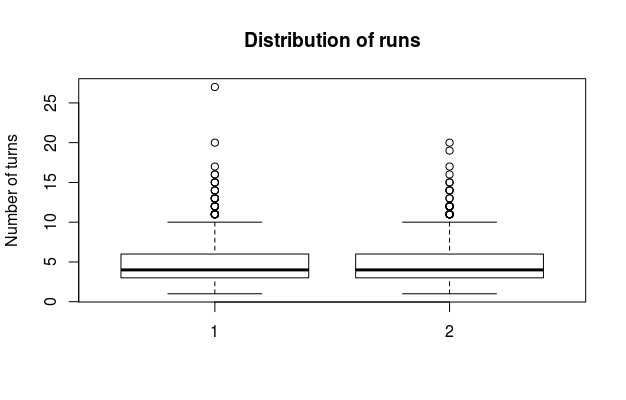
\includegraphics[width=10cm,height=10cm,keepaspectratio]{imgs/box-sqrt-fif.png}\\
\caption{Comparing the dynamic interval with $a$ and $b$ being 0.15}
\end{figure}

Using the static interval for emission probabilities the accuracy of the whole model and the forward algorithm can be calculated. Doing 1,000 runs again the times that the algorithm predicts the right node is $\sim68.64\%$. With a weighted accuracy, where locality is taken into account as defined in equation \ref{eq:accuracy}, the accuracy is $\sim82.79\%$. The accuracy of every prediction is summed up and divided by the number of predictions to get that result.
\begin{equation}\label{eq:accuracy}
\begin{split}
\mathtt{distance(n_{croc}, n_{prediction})}=d, \; \mathtt{the \; distance \; between \; two \; nodes.}
\\
\mathtt{accuracy(n_{prediction})} = 1 / d, \; \mathtt{if} \; d > 0 \hspace{151pt}
\\
\mathtt{accuracy(n_{prediction})} = 1, \; \mathtt{if} \; d = 0 \hspace{163pt}
\end{split}
\end{equation}

\subsection{Different path finding algorithms}
%Different path finding algorithms: A*, (Dijkstra), modified DFS.

The two different path finding algorithms used were the modified DFS described in \ref{sec:implementation} and A*. Finding a good heuristic proved to be difficult and there were problems of the algorithm going in circles at times. The average time to calculate the optimal path took $\sim8$ seconds for A*. The modified DFS is much faster with an average of $\sim245$ milliseconds.


\section{Discussion}

The average number of moves in the result clearly speak for themselves. The way the transition and emission probabilities were represented clearly made the forward algorithm undoubtedly effective. There certainly is room for more improvement in the approximation of the emission probabilities and other strategies, but the current implementation is still working extremely well.

One area that could be improved are strategies relating to selecting the best route. At the start of the program, the forward algorithm will have less information to go on and be less accurate. To counteract that and minimize the number of unnecessary moves in the beginning, the path algorithm could go towards the middle of the grid during the first couple of moves if the predicted node is not too far away. This fixes a problem where the ranger would sometimes go forwards and backwards in the graph. Another strategy that could be employed is to take routes that cumulatively have higher probability of the crocodile being there, instead of only looking at the node with the highest probability.

Another part of the path finding that could be improved is the algorithm for finding the shortest path. The algorithm is quite expensive time complexity wise and could be improved by using Dijkstra's algorithm.

%Also the strategy could be improved, as the first two predictions of the forward algorithm often are wrong. One such strategy would be to during the first two moves, only go to the predicted destination if its within a two move range. Otherwise go towards the middle of the graph, ex. node 25. This minimizes the unnecessary moves that often are done at the beginning of the game.

\section{Conclusion}

Do we need any?

Yes

\end{document}
